\documentclass[fleqn]{article}
\usepackage[nodisplayskipstretch]{setspace}
\usepackage{amsmath, nccmath}
\usepackage{amssymb}
\usepackage{enumitem}
\usepackage{matlab-prettifier}
\usepackage{scalerel}
\usepackage{graphicx}
\usepackage{float}
\usepackage{changepage}
\usepackage{environ,capt-of}

\newcommand{\zerodisplayskip}{
	\setlength{\abovedisplayskip}{0pt}%
	\setlength{\belowdisplayskip}{0pt}%
	\setlength{\abovedisplayshortskip}{0pt}%
	\setlength{\belowdisplayshortskip}{0pt}%
	\setlength{\mathindent}{0pt}}
	
\let\oldfigure\figure% Store original figure float environment
\let\endoldfigure\endfigure
\RenewEnviron{figure}[1][H]{% Update figure environment
  %\par\vspace{\intextsep}% Assume in-text placement, so insert appropriate vertical spacing
  \noindent
  % \patchcmd{<cmd>}{<search>}{<replace>}{<success>}{<failure>}
  \patchcmd{\BODY}{\caption}{\captionof{figure}}{}{}% Replace \caption with \captionof{figure} inside \BODY
  % Set "figure"
  \begin{minipage}{\linewidth}
    \BODY
  \end{minipage}
  %\par\vspace{\intextsep}% Assume in-text placement, so insert appropriate vertical spacing
}

\title{Homework 5}
\author{Owen Sowatzke}
\date{November 16, 2023}

\begin{document}
	\offinterlineskip
	\setlength{\lineskip}{12pt}
	\zerodisplayskip
	\maketitle
	
	\begin{enumerate}[nolistsep]
		\item Design a discrete-time second-order Butterworth lowpass filter with cutoff frequency equivalent to $f_c = 1.6 \text{kHz}$. Assume the ADC sampling frequency is $f_s = 8 \text{kHz}$. Use the impulse invariance method with $T_d = 1$.
		
			\begin{enumerate}[nolistsep]
				\item Calculate the cutoff frequency for the desired digital filter (i.e., convert the analog specs to digital specs.)
				
					\begin{equation*}
						\omega_c = \frac{2{\pi}f_c}{f_s} = \frac{2{\pi}(1.6\ \text{kHz})}{8\ \text{kHz}} = \mathbf{0.4\pi}
					\end{equation*}
					
				\item Calculate the cutoff frequency for the prototype analog filter.
				
					\begin{equation*}
						\Omega_c = \frac{\omega_c}{T_d} = \mathbf{0.4\pi} 
					\end{equation*}
					
				\item Derive the transfer function $H_a(s)$ for the prototype analog filter by selecting the left-half-plane poles of $H_a(s)H_a(-s)$. Show your work. Show that this matched the result of the following MATLAB command:
				
				\texttt{[bs, as] = butter(N,$\Omega_c$,'low','s')}
				
				\begin{equation*}
					H_a(s)H_a(-s) = \frac{(-1)^N{\Omega_c}^{2N}}{s^{2N} + (-1)^N{\Omega_c}^{2N}}
				\end{equation*}
				
				\begin{equation*}
					= \frac{(-1)^2(0.4\pi)^4}{s^4 + (-1)^4(0.4\pi)^4} = \frac{(0.4\pi)^4}{s^4 + (0.4\pi)^4}
				\end{equation*}
				
				Solve for the poles of the above expression:
				
				$s^4 + (0.4\pi)^4 = 0$
				
				$\Rightarrow s^4 = -(0.4\pi)^4$
				
				$\Rightarrow s^4 = (0.4\pi)^4e^{j\pi}$
				
				$\Rightarrow s^4 = (0.4\pi)^4e^{j(\pi + 2{\pi}k)}\ \forall\ k \in \mathbb{Z}$
				
				$\Rightarrow s = 0.4{\pi}e^{j({\pi/4} + {\pi}k/2)}\ \forall\ k \in \mathbb{Z}$
				
				$\therefore$ $H_a(s)H_a(-s)$ has 4 unique poles:
				
				$s_1 = 0.4{\pi}e^{j{\pi}/4}$
				
				$s_2 = 0.4{\pi}e^{j3{\pi}/4}$
				
				$s_3 = 0.4{\pi}e^{-j3{\pi}/4}$
				
				$s_4 = 0.4{\pi}e^{-j{\pi}/4}$
				
				Because the filter is stable, the poles of $H_a(s)$ must be in the LHP.
				
				$\therefore$ $H_a(s)$ has two poles:
				
				$s_1 = 0.4{\pi}e^{j3{\pi}/4}$
				
				$s_2 = 0.4{\pi}e^{-j3{\pi}/4}$
				
				Now, we can rewrite $H_a(s)$ in the following form:
				
				\begin{equation*}
					H_a(s) = \frac{(0.4\pi)^2}{(s - 0.4{\pi}e^{j3{\pi}/4})(s - 0.4{\pi}e^{-j3{\pi}/4})}
				\end{equation*}
				
				\begin{equation*}
					= \frac{(0.4\pi)^2}{s^2 - (0.4{\pi}e^{j3{\pi}/4} + 0.4{\pi}e^{-j3{\pi}/4})s + (0.4\pi)^2}
				\end{equation*}
				
				\begin{equation*}
					= \frac{(0.4\pi)^2}{s^2 - 0.8\pi\cos(3\pi/4)s + (0.4\pi)^2}
				\end{equation*}
				
				\begin{equation*}
					\mathbf{= \frac{1.5791}{s^2 + 1.7772s + 1.5791}}
				\end{equation*}
				
				\pagebreak
				We can compare this transfer function to the output of the following MATLAB command:
				
				\begin{figure}[H]
					\centerline{\fbox{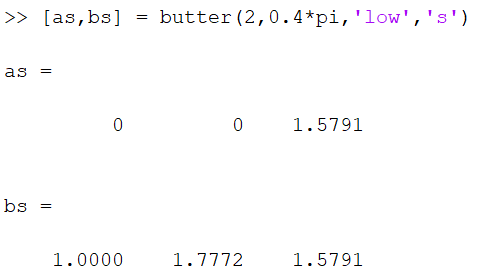
\includegraphics[width=0.5\textwidth]{prob_1c.png}}}
					\caption{Using MATLAB to Solve for $H_a(s)$}
				\end{figure}
				
				The transfer function $H_a(s)$ derived using MATLAB has numerator polynomial of $0s^2 + 0s + 1.5791 = 1.5971$ and a denominator polynomial of $s^2 + 1.7772s + 1.5791$. Note that this is equivalent to the transfer function that was analytically derived.
				
				\item Derive the transfer function $H(z)$ for the desired digital filter. Also show the result of the following MATLAB command, which gives the coefficients for the final, simplified $H(z)$:
				
				\texttt{[bz, az] = impinvar(bs,as,$1/T_d$)}
				
				We first need to find $h_a(t)$ by taking an inverse Laplace transform of $H_a(s)$. Start by using partial fraction expansion to write $H_a(s)$ in the following form:
				
				\begin{equation*}
					H_a(s) = \frac{A_1}{s - 0.4{\pi}e^{j3{\pi}/4}} +  \frac{A_2}{s - 0.4{\pi}e^{-j3{\pi}/4}}
				\end{equation*}
				
				\begin{equation*}
					A_1 = H_a(s)(s - 0.4{\pi}e^{j3{\pi}/4}) = \left.\frac{(0.4\pi)^2}{s - 0.4{\pi}e^{-j3{\pi}/4}}\right\vert_{s = 0.4{\pi}e^{j3{\pi}/4}}
				\end{equation*}
				
				\begin{equation*}
					= \frac{(0.4\pi)^2}{0.4{\pi}e^{j3{\pi}/4} - 0.4{\pi}e^{-j3{\pi}/4}} = \frac{(0.4\pi)^2}{j0.8{\pi}\sin(3\pi/4)}
				\end{equation*}
				
				\begin{equation*}
					 = \frac{(0.4\pi)}{j2(1/\sqrt{2})} = -\frac{j\pi\sqrt{2}}{5}
				\end{equation*}
				
				\begin{equation*}
					A_2 = H_a(s)(s - 0.4{\pi}e^{-j3{\pi}/4}) = \left.\frac{(0.4\pi)^2}{s - 0.4{\pi}e^{j3{\pi}/4}}\right\vert_{s = 0.4{\pi}e^{-j3{\pi}/4}}
				\end{equation*}
				
				\begin{equation*}
					= \frac{(0.4\pi)^2}{0.4{\pi}e^{-j3{\pi}/4} - 0.4{\pi}e^{j3{\pi}/4}} = \frac{(0.4\pi)^2}{-j0.8{\pi}\sin(3\pi/4)}
				\end{equation*}
				
				\begin{equation*}
					 = \frac{(0.4\pi)}{-j2(1/\sqrt{2})} = \frac{j\pi\sqrt{2}}{5}
				\end{equation*}
				
				\begin{equation*}
					H_a(s) = \frac{-j\pi\sqrt{2}}{5}\left(\frac{1}{s - 0.4{\pi}e^{j3\pi/4}}\right) + \frac{j\pi\sqrt{2}}{5}\left(\frac{1}{s - 0.4{\pi}e^{-j3\pi/4}}\right)
				\end{equation*}
				
				\begin{equation*}
					= \frac{-j\pi\sqrt{2}}{5}\left(\frac{1}{s - 0.4{\pi}\left(-\frac{1}{\sqrt{2}} + \frac{j}{\sqrt{2}}\right)}\right)
				\end{equation*}
				
				\begin{equation*}
					 + \frac{j\pi\sqrt{2}}{5}\left(\frac{1}{s - 0.4{\pi}\left(-\frac{1}{\sqrt{2}} - \frac{j}{\sqrt{2}}\right)}\right)
				\end{equation*}
				
				Now take the inverse Laplace transform to get $h_a(t)$.
				
				\begin{equation*}
					h_a(t) = \frac{-j\pi\sqrt{2}}{5}e^{0.4\pi\left(-\frac{1}{\sqrt{2}} + \frac{j}{\sqrt{2}}\right)t}u(t) + \frac{j\pi\sqrt{2}}{5}e^{0.4\pi\left(-\frac{1}{\sqrt{2}} - \frac{j}{\sqrt{2}}\right)t}u(t)
				\end{equation*}
				
				\begin{equation*}
					= \frac{\pi\sqrt{2}}{5}e^{-\frac{0.4{\pi}t}{\sqrt{2}}}\left(-je^{\frac{j0.4{pi}t}{\sqrt{2}}} + je^{-j\frac{0.4{\pi}t}{\sqrt{2}}}\right)u(t)
				\end{equation*}
				
				\begin{equation*}
					= \frac{2\pi\sqrt{2}}{5}e^{-\frac{0.4{\pi}t}{\sqrt{2}}}\left(\frac{e^{\frac{j0.4{\pi}t}{\sqrt{2}}} - e^{-\frac{j0.4{\pi}t}{\sqrt{2}}}}{j2}\right)u(t)
				\end{equation*}
				
				\begin{equation*}
					 = \frac{2\pi\sqrt{2}}{5}e^{-\frac{0.4{\pi}t}{\sqrt{2}}}\sin{\left(\frac{0.4{\pi}t}{\sqrt{2}}\right)}u(t)
				\end{equation*}
				
				Now sample $h_a(t)$ to obtain $h[n]$:
				
				\begin{equation*}
					h[n] = \frac{2\pi\sqrt{2}}{5}e^{-\frac{0.4{\pi}n}{\sqrt{2}}}\sin{\left(\frac{0.4{\pi}n}{\sqrt{2}}\right)}u[n]
				\end{equation*}
				
				Use the following z-transform pair to obtain $H(z)$
				
				\begin{equation*}
					r^{n}sin({\omega_0}n)u[n] \leftrightarrow \frac{rsin(\omega_0)z^{-1}}{1 - 2rcos(\omega_0)z^{-1} + r^{2}z^{-2}}\quad |z| > r
				\end{equation*}
				
				\begin{equation*}
					H(z) = \frac{2\pi\sqrt{2}}{5}\left(\frac{e^{-\frac{0.4\pi}{\sqrt{2}}}\sin{\left(\frac{0.4\pi}{\sqrt{2}}\right)z^{-1}}}{1 - 2e^{-\frac{0.4\pi}{\sqrt{2}}}\cos{\left(\frac{0.4\pi}{\sqrt{2}}\right)}z^{-1} + e^{-\frac{0.8\pi}{\sqrt{2}}}z^{-2}}\right)
				\end{equation*}
				
				\begin{equation*}
					\mathbf{= \frac{0.5673z^{-1}}{1 - 0.5186z^{-1} + 0.1691z^{-2}}}
				\end{equation*}
				
				We can compare this transfer function to the output of the following MATLAB command, where \texttt{bs} and \texttt{as} are derived are derived using the MATLAB code given in part (c):
				
				\begin{figure}[H]
					\centerline{\fbox{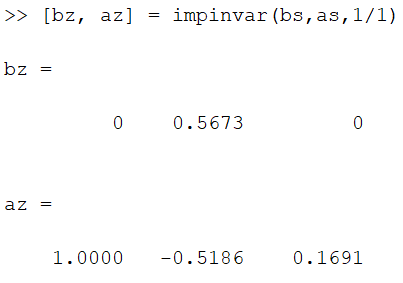
\includegraphics[width=0.5\textwidth]{prob_1d.png}}}
					\caption{Using MATLAB to Solve for $H(z)$}
				\end{figure}
				
				The transfer function $H(z)$ derived using MATLAB has numerator polynomial of $0z^{-2} + 0.5673z^{-1} + 0z^{-2} = 0.5673z^{-1}$ and a denominator polynomial of $1 - 0.5186z^{-1} + 0.1691z^{-2}$. Note that this is equivalent to the transfer function that was analytically derived.
				
			\item Derive the difference equation (LCCDE) that we would use to implement the filter.
			
				$Y(z)(1 - 0.5186z^{-1} + 0.1691z^{-2}) = X(z)(0.5673z^{-1})$
				
				$y[n] - 0.5186y[n-1] + 0.1691y[n-2] = 0.5673x[n-1]$
				
				$\mathbf{y[n] = 0.5186y[n-1] - 0.1691y[n-2] + 0.5673x[n-1]}$
				
			\item Plot the frequency response as follows:
			
				\texttt{[H,w] = freqz(bz,az)}
				
				\texttt{semilogy(w/pi,abs(H))}
				
				\begin{figure}[H]
					\centerline{\fbox{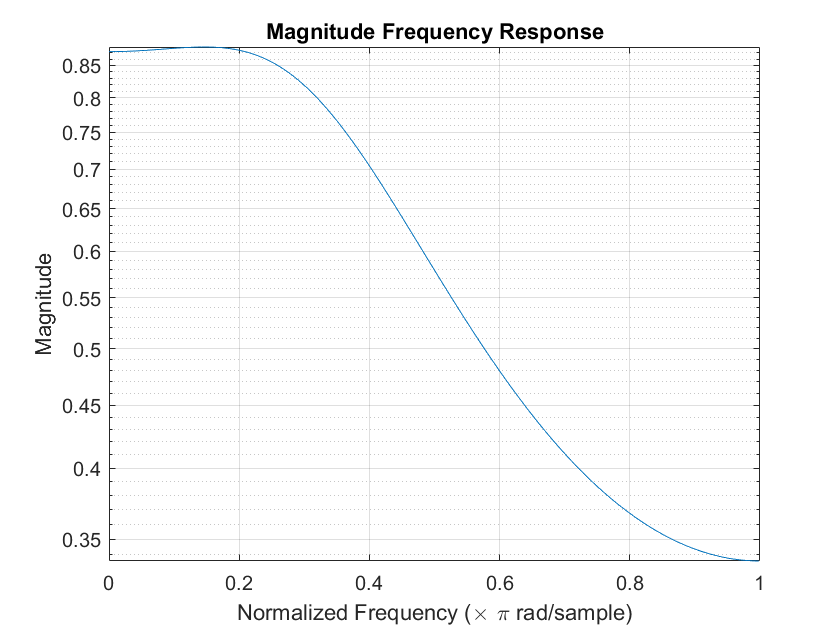
\includegraphics[width=0.5\textwidth]{prob_1f.png}}}
					\caption{Magnitude Frequency Response}
				\end{figure}
				
			\item What is the approximate magnitude frequency response at zero frequency? How can we modify the filter to achieve unit magnitude frequency response at zero frequency? Optional can you determine a way to modify the filter that will achieve unit magnitude frequency response at zero frequency without affecting the frequency response at other frequencies?
			
				The magnitude frequency response at zero frequency is approximately $0.871994$. To achieve a unit magnitude frequency response at zero frequency we want to scale the transfer function by $1/0.871994 = 1.1468$. This is equivalent to scaling the numerator of the transfer function, \texttt{bz}, by $1.1468$. This modified filter can be implemented with the following LCCDE:
				
				$y[n] = 0.5186y[n-1] - 0.1691y[n-2] + 0.6506x[n-1]$
		\end{enumerate}
		\item Design a discrete-time second-order Butterworth lowpass filter with cutoff frequency $\omega_c = 0.4\pi\ \text{rad}$. Use the impulse invariance method.
			Hint: This problem is trivial after you've completed the previous problem.
		\pagebreak
		\item Design a discrete-time second-order Butterworth lowpass filter with cutoff frequency equivalent to $f_c = 1.6\ \text{kHz}$. Assume the ADC sampling frequency is $f_s = 8 \text{kHz}$. Use the bilinear transformation methods with $T_d = 2$.
		\begin{enumerate}
			\item Calculate the cutoff frequency for the desired digital filter (i.e., convert the analog specs to digital specs.)
			\begin{equation*}
				\omega_c = \frac{2{\pi}f_c}{f_s} = \frac{2{\pi}(1.6\ \text{kHz})}{8\ \text{kHz}} = \mathbf{0.4\pi}
			\end{equation*}
			\item Calculate the cutoff frequency for the prototype analog filter.
			\begin{equation*}
				\Omega_c = \frac{\omega_c}{T_d} = \frac{0.4\pi}{2} = \mathbf{0.2\pi} 
			\end{equation*}
		\end{enumerate}
	\end{enumerate}
\end{document}
